\documentclass[a4paper,12pt]{book}
\usepackage[spanish]{babel}
\usepackage[utf8]{inputenc}
\usepackage{graphicx}
\usepackage{titling}
\usepackage{makeidx} % Paquete para el índice
\usepackage{fontspec}
\usepackage{tabularx}
\usepackage[acronym,nonumberlist,nopostdot]{glossaries}
\setmainfont{Noto Sans CJK KR}



\title{HwaRangDo: El Camino de los Hombres Florecientes}
\author{Tú Nombre}
\date{\today}

\makeindex % Inicializar el índice


\begin{document}

	\begin{titlepage}
		\centering
		\vspace*{\fill}
		
\includegraphics[width=0.7\textwidth]{images/sam_taeguk.png} % Reemplaza 'hwarangdo_logo' con el nombre de tu archivo de logotipo
		\vspace*{\fill}

		\vspace*{2cm}

		{\Huge\bfseries HwaRangDo: El Camino de los Hombres Flores\par}
		\vspace{2cm}
		{\Large Tú Nombre\par}

		\vspace*{\fill}
		{\large \today\par}
	\end{titlepage}

	\tableofcontents
	% Índice generado automáticamente|

	\frontmatter % Cambia al estilo de numeración de páginas romanos para las partes iniciales

	%	El archivo entre {} debe ser \invlude{/ruta/al/nombredelarchivo} y el archivo tiene que tener .tex


	%\chapter*{Prólogo}
%Un sueño comienza a convertirse en realidad cuando uno invierte todo su corazón y pasión en aquello que ama. A veces, esto puede parecer ilógico, pero con la ayuda del Padre (como se menciona en San Juan 3:16), nada es imposible. No hay mayor ceguera que la de aquel que se niega a ver, ni mayor sordera que la de aquel que se niega a escuchar.
%
%Este libro tiene como objetivo registrar los logros y la historia de nuestras academias, dejando una marca indeleble en el tiempo. La vida es efímera, y lo que somos hoy puede convertirse en un recuerdo mañana. Lamentablemente, muchos han pasado por este mundo sin dejar un legado duradero.
%
%Por lo tanto, te animo a seguir explorando nuestro sistema de Ninjitsu Coreano - Sulsa, que abarca tanto la defensa personal integral como las disciplinas marciales de contacto. Como se dice, ``El guerrero Hwarang Sulsa es como el ave fénix que renace de sus cenizas'', y este libro es un testimonio de esa resiliencia y perseverancia.
%
%\mainmatter % Cambia al estilo de numeración de páginas arábigos para el contenido principal

\chapter{Prólogo}
El tiempo es un tejido frágil y efímero que todos, de una forma u otra, tejemos a lo largo de nuestras vidas. En ese intrincado tapiz, las huellas de las personas se entrelazan con las obras que dejan atrás, definiendo así su legado. Cada paso que damos, cada elección que tomamos, y cada obra que creamos son hilos que contribuyen a esta compleja narrativa.

En el camino de la vida, algunos eligen caminar con un propósito ardiente, entregando su corazón y su pasión a un arte, una disciplina que trasciende el tiempo. El Hwarangdo\textregistered, un antiguo arte marcial coreano, es un claro ejemplo de esta dedicación apasionada. Es un compromiso con la perfección, no solo en las técnicas de combate, sino también en la forja del carácter humano.

Este libro es un testimonio de la historia y el espíritu del Hwarangdo\textregistered, una herencia que se ha transmitido a lo largo de las generaciones. En sus páginas, encontrarás la sabiduría de quienes han dedicado su vida a esta disciplina, y comprenderás que el Hwarangdo\textregistered va más allá de las artes marciales; es una filosofía de vida. Poner todo el corazón en el entrenamiento es la esencia misma de este arte.

Los guerreros Hwarang del pasado, como aquellos que siguen el camino hoy en día, comprendieron que la excelencia en cualquier esfuerzo requiere un compromiso total. Más allá de la destreza en el combate, el Hwarangdo\textregistered promueve valores fundamentales: lealtad, honestidad, valentía y compasión. Estos valores son los pilares sobre los cuales se erige el guerrero Hwarang.

El Hwarangdo\textregistered es como un ave fénix que renace de sus cenizas, y este libro es un reflejo de esa resiliencia y determinación. A medida que exploras sus páginas, te sumergirás en una tradición rica y antigua que sigue viva en el mundo contemporáneo. Un legado que te desafía a poner todo tu corazón en tu entrenamiento, a perseguir tus sueños y a dejar tu propia huella en la historia.

Así que te invito a que continúes descubriendo y abrazando nuestro sistema de Ninjitsu Coreano - Sulsa, una disciplina que abarca la defensa personal integral y los deportes de contacto marcial. Al hacerlo, estarás contribuyendo a la historia en la que todos somos autores, y tus obras se convertirán en una realidad perdurable en el tejido del tiempo.

Que este libro sea tu guía en el viaje del Hwarangdo\textregistered y que, al igual que aquellos que vinieron antes, encuentres en él la inspiración para dar lo mejor de ti y hacer realidad tus sueños más profundos.

\mainmatter % Cambia al estilo de numeración de páginas arábigos para el contenido principal
	\chapter{Contexto Histórico}
\section{Época de los Tres Reinos de la península coreana}

La \textbf{época de los Tres Reinos} en Corea es un período histórico crucial que se extendió desde aproximadamente el siglo I hasta el siglo VII d.C. Durante este tiempo, la península coreana estaba dividida en tres reinos principales, cada uno con sus propias características y contribuciones a la historia y cultura de Corea.

\begin{figure}[h]
	\centering
	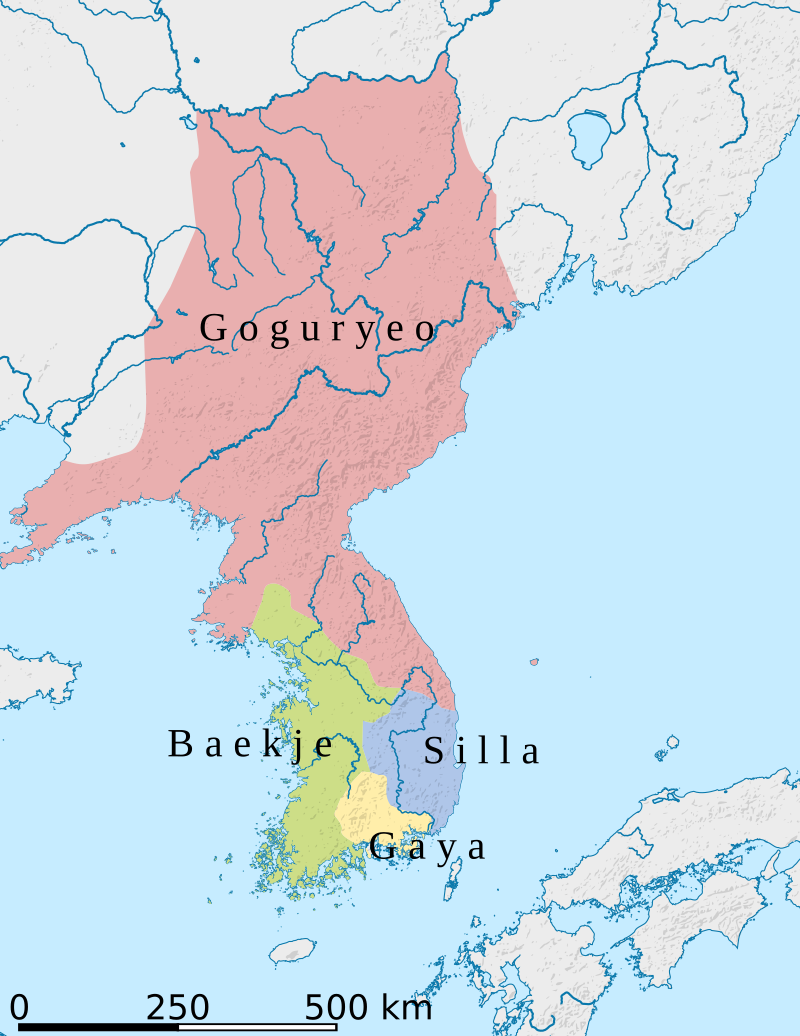
\includegraphics[width=0.3\textwidth]{images/Historia/mapa_tres_reinos.png} % Reemplaza 'mapa_corea' con el nombre de tu archivo de imagen
	\caption{Mapa de Corea con los Tres Reinos}
\end{figure}

\subsection{Goguryeo}

Goguryeo fue el reino más septentrional y poderoso de los Tres Reinos. Su capital estaba ubicada en la actual región norcoreana. Goguryeo mantuvo una fuerte influencia militar y política en la península, y se caracterizó por su habilidad para resistir las invasiones chinas de la dinastía Han y luego de la dinastía Tang. Este reino desarrolló una cultura propia y estableció una gran parte de lo que hoy es Corea del Norte.

\subsection{Baekje}

Baekje ocupó la región suroeste de la península coreana, con su capital en lo que hoy es la ciudad de Seúl. Este reino tenía estrechos vínculos culturales y comerciales con China y Japón, lo que le permitió adoptar y difundir la influencia budista en la península. Baekje fue conocido por su avanzada cultura y arte, y contribuyó significativamente al desarrollo de la cultura coreana.

\subsection{Silla}

Silla, ubicado en la región sureste de Corea con su capital en Gyeongju, fue el último de los Tres Reinos en unificarse bajo un gobierno centralizado. Silla es famoso por su sistema de gobierno estable y su énfasis en la educación y la cultura. Durante esta época, se estableció el sistema de exámenes gubernamentales basado en el conocimiento confuciano, que influyó en gran medida en la administración pública de Corea durante siglos.

A medida que avanzaba la época de los Tres Reinos, se produjo una serie de conflictos y alianzas cambiantes entre los reinos, con episodios de unificación temporal y fragmentación. Finalmente, en el siglo VII, Silla logró unificar la península coreana bajo su dominio y estableció el período conocido como el ''Silla Unificado``. Este período dio paso a una mayor estabilidad y desarrollo cultural en Corea antes de la llegada de la dinastía Goryeo. La época de los Tres Reinos dejó un profundo legado en la historia y la cultura de Corea, con influencias que perduran hasta el día de hoy.

\section{Hwarang}

Los \textbf{Hwarang}, también conocidos como ''Hwa Rang`` o ''Hwarangdo\textregistered``, fueron un grupo de jóvenes guerreros aristocráticos en la antigua Corea. Su existencia se sitúa en los períodos de los Tres Reinos y la posterior dinastía Silla, que abarcan los siglos VI al X d.C. Estos guerreros eran conocidos no sólo por su habilidad en el combate, sino también por su énfasis en la educación, la moral, la cultura y las artes.

\begin{figure}[h]
	\centering
	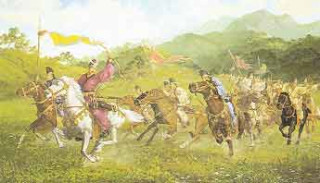
\includegraphics[width=0.3\textwidth]{images/Historia/pintura_hrd.jpg} % Reemplaza 'mapa_corea' con el nombre de tu archivo de imagen
	\caption{Grupo élite de Corea}
\end{figure}


\subsubsection{Origen y Significado}

La palabra ''Hwarang`` se traduce aproximadamente como ``caballeros de la flor'' o ``juventud floreciente''. Eran un grupo selecto de jóvenes nobles que se sometían a un entrenamiento riguroso tanto en artes marciales como en aspectos culturales y éticos.

\subsubsection{Educación Integral}

Los Hwarang no solo se entrenaban en técnicas de combate, sino que también recibían una educación completa que incluía poesía, música, filosofía y moral. Este enfoque en la educación y la cultura los diferenciaba de otros guerreros de la época.

\subsubsection{Código de Ética}

\begin{table}[t]
	\caption{Código Hwarang}
	\begin{center}
		\begin{tabular}{ | m{2cm} | m{5cm} | m{5cm} | }
			\hline Número & Hangul & Traducción \\ \hline
			Il & 사군이충: Sa Gun I Chung & Lealtad a nuestra Patria \\
			I & 사친이효: Sa Chin I Hyo & Lealtad a nuestros padres y maestros \\
			Sam & 교우이신: Gyo U I Sin & Confianza y hermandad entre amigos\\
			Sa & 임전무퇴: Im Jeon Mu Toe & Coraje para no retroceder frente al enemigo\\
			O & 살생유택: Sal Saeng Yu Taek & Justicia para no tomar una vida sin causa\\ \hline
		\end{tabular}
	\end{center}
\end{table}


Los Hwarang seguían un estricto código de ética conocido como ''Hwarangdo\textregistered``, que promovía valores como la lealtad, la rectitud, la valentía y la integridad. Este código tenía como objetivo formar no solo guerreros hábiles, sino también líderes virtuosos.

El fervor de los Hwarang ayudó a que Silla se convirtiera en la primera ''Tierra de Buda`` del mundo y condujo a la unificación de los tres reinos de Corea. Los principios budistas estaban tan arraigados en el código de los Hwarang que un gran número de monjes participaba en el Hwarang-Do, y durante tiempos de guerra, se despojaban de sus hábitos y tomaban las armas para morir por Silla.

El código Hwarang fue establecido en el trigésimo año del reinado del Rey Chin-Hung. Dos destacados guerreros Hwarang, Kwi-San y Ch'u-Hang, buscaron al famoso guerrero y monje budista Wong-Gwang Popsa en el Templo Kusil en la Montaña Unmun y le pidieron que les diera mandamientos que los hombres pudieran seguir y que no abrazaran la vida recluida de un monje budista.

\begin{figure}[h]
	\centering
	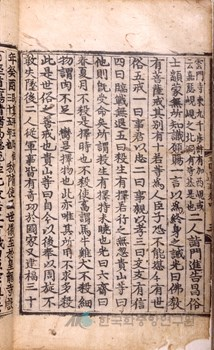
\includegraphics[width=0.4\textwidth]{images/Historia/codigo_hwarang.jpg} % Reemplaza 'mapa_corea' con el nombre de tu archivo de imagen
	\caption{Las Cinco Reglas Seculares de la Escuela de Wongwang en la época de los 3 reinos}
\end{figure}

Los mandamientos, basados en principios confucianos y budistas, se dividieron en el Código de las cinco reglas Hwarang y las nueve virtudes. Estos principios no eran tomados a la ligera por los Hwarang.


\begin{table}[t]
	\caption{Nueve Virtudes}
	\begin{center}
		\begin{tabular}{ | m{2cm} | m{5cm} | }
			\hline Hangul & Traducción \\ \hline
			인: In & Humanidad \\
			의: Ui & Justicia \\
			예: Ye & Cortesía \\
			지: Ji & Sabiduría \\
			신: Sin & Confianza \\
			선: Seon & Bondad \\
			덕: Deok & Virtud \\
			충: Chung & Lealtad \\
			용: Yong & Coraje \\

			\hline
		\end{tabular}
	\end{center}
\end{table}


El fervor de los Hwarang ayudó a que Silla se convirtiera en la primera "Tierra de Buda" del mundo y condujo a la unificación de los tres reinos de Corea. Los principios budistas estaban tan arraigados en el código de los Hwarang que un gran número de monjes participaban en el Hwarang-Do, y durante tiempos de guerra, se despojarían de sus hábitos y tomarían las armas para morir por Silla.

\subsubsection{Artes Marciales}

Aunque se destacaban en la educación y la cultura, los Hwarang también eran conocidos por su habilidad en el combate. Dominaban varias formas de artes marciales y estaban preparados para defender su reino en caso de guerra.

\subsubsection{Contribución a la Unificación de Silla}

Durante el período de los Tres Reinos en Corea, Silla se convirtió en uno de los reinos más poderosos. Se dice que los Hwarang desempeñaron un papel crucial en la unificación de Silla y en la posterior estabilidad del reino.

\subsubsection{Legado Cultural}

La influencia de los Hwarang perduró en la cultura coreana a lo largo de la historia. Su énfasis en la educación, la ética y la excelencia en las artes marciales influyó en la formación de la cultura y la identidad coreanas.

Los Hwarang son un ejemplo único en la historia de las sociedades guerreras, ya que combinaron la destreza en el combate con un profundo compromiso con la educación y los valores morales. Su legado sigue siendo un símbolo importante de la historia y la cultura coreanas.


%\begin{figure}[h]
%	\centering
%
%	\subfloat[Imagen 1]{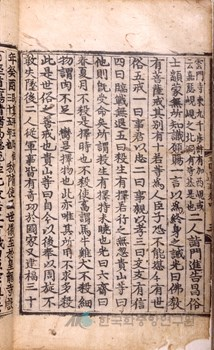
\includegraphics[width=0.2\textwidth]{images/Historia/codigo_hwarang.jpg}}\hspace{1cm}
%	\subfloat[Imagen 2]{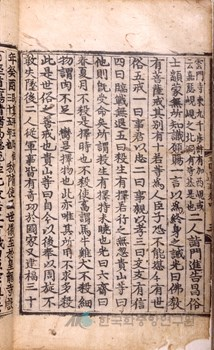
\includegraphics[width=0.2\textwidth]{images/Historia/codigo_hwarang.jpg}}\hspace{1cm}
%	\subfloat[Imagen 3]{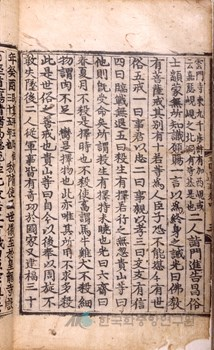
\includegraphics[width=0.2\textwidth]{images/Historia/codigo_hwarang.jpg}}\hspace{1cm}
%	\subfloat[Imagen 4]{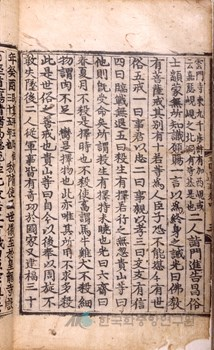
\includegraphics[width=0.2\textwidth]{images/Historia/codigo_hwarang.jpg}}\hspace{1cm}
%	\subfloat[Imagen 5]{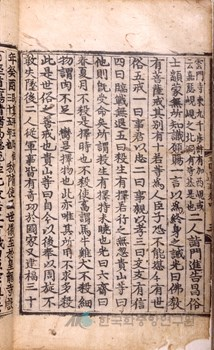
\includegraphics[width=0.2\textwidth]{images/Historia/codigo_hwarang.jpg}}
%
%	\caption{Secuencia Patada Frontal}
%
%\end{figure}

	%	\chapter{Introducción}

En el apasionante mundo de las artes marciales, el Hwarangdo\textregistered brilla con una singularidad que ha resistido el paso del tiempo. Este manual te sumergirá en las profundidades de este ancestral sistema de combate coreano y te servirá como un invaluable recordatorio de sus técnicas y principios fundamentales.
El HwaRangDo\textregistered, (hangul
\footnote[1]{Alfabeto nativo coreano (en contraste con los hanja, o caracteres chinos).1​ Cada bloque silábico hangul consiste en alguno de los 24 fonemas (jamo): 14 consonantes y 10 vocales. Históricamente, tenía 3 consonantes y una vocal más.
Estos bloques silábicos pueden ser escritos tanto horizontalmente, de izquierda a derecha, como verticalmente, de arriba hacia abajo, con las columnas dispuestas de derecha a izquierda.} (coreano): 화랑도;
hanja \footnote[2]{Nombre que reciben los sinogramas
en coreano pero, de forma más específica, se refiere a
los caracteres chinos que los coreanos tomaron prestados
e incorporaron a su idioma, cambiando su pronunciación} (chino): 花郞道) cuyo nombre se traduce como ``El Sendero de los Caballeros Florecientes'', es más que una mera disciplina física; es un camino hacia la autotrascendencia y el equilibrio entre el cuerpo, la mente y el espíritu. Este libro está diseñado para aquellos que desean explorar y recordar los secretos de este arte marcial, y para quienes buscan aplicar sus enseñanzas en la vida cotidiana.

A medida que navegues por las páginas de este manual, te sumergirás en la rica historia de los Hwarang, una orden de guerreros que floreció en la antigua Corea y sentó las bases de este arte. Descubrirás sus valores esenciales, sus códigos de honor y cómo estos principios siguen siendo relevantes en la práctica contemporánea del Hwarangdo\textregistered.

Este libro te llevará paso a paso a través de las técnicas de combate, las posturas fundamentales y las formas de movimiento característicos del Hwarangdo\textregistered. Cada página es una guía práctica que te recordará cómo ejecutar golpes precisos, patadas fluidas y bloqueos seguros, así como cómo aplicar las habilidades de defensa personal en situaciones reales.

El propósito de este manual es servir como un compañero constante en tu viaje en el camino de los Caballeros Flor. Ya sea que seas un principiante que busca fortalecer sus bases o un practicante experimentado que necesita un recordatorio, encontrarás en estas páginas una valiosa fuente de conocimiento y una inspiración para continuar perfeccionando tu arte.

Así que, te invitamos a sumergirte en este viaje, a recordar y redescubrir las enseñanzas del Hwarangdo\textregistered, y a aplicarlas en tu vida diaria. Este manual es tu guía confiable en el sendero de los Caballeros Flor, una herramienta esencial que te recordará que la excelencia se encuentra en la práctica constante y la búsqueda de la perfección. ¡Bienvenido al mundo del Hwarangdo\textregistered y a la aventura que te espera en estas páginas!
	%	\include{faja_blanca}
	%	\include{faja_celeste}
	%	\include{faja_celeste_amarillo}
	%	\include{faja_amarillo}
	%	\include{faja_amarillo_verde}
	%	\include{faja_verde}
	%	\include{faja_verde_azul}
	%	\include{faja_azul}


\end{document}